% Lab 7 implementation paper — DRAFT v0.2 (24 Oct 2026; revised after self-review, see Prompt 16), written BEFORE any real model result.
% Compiles with IEEEtran (Overleaf) and falls back to a two-column article class where IEEEtran is absent.
% Every number from a model run comes from paper/results_tables.tex, generated by scripts/make_paper_tables.py.
% Markers: [PENDING] = needs real results; [TO VERIFY] = fact not yet checked against its source or run.
\IfFileExists{IEEEtran.cls}{\documentclass[conference]{IEEEtran}}{\documentclass[10pt,twocolumn]{article}\usepackage[margin=0.75in]{geometry}}
\usepackage[T1]{fontenc}
\usepackage{graphicx,booktabs,amsmath,xcolor,url}
\usepackage[hidelinks]{hyperref}
\providecommand{\IEEEkeywords}{}
\makeatletter\@ifundefined{IEEEauthorblockN}{\newcommand{\IEEEauthorblockN}[1]{#1}\newcommand{\IEEEauthorblockA}[1]{\\{\small #1}}}{}\makeatother
\newcommand{\pending}[1]{\textcolor{red}{[PENDING: #1]}}
\newcommand{\toverify}[1]{\textcolor{orange}{[TO VERIFY: #1]}}

\title{Does the Virtual Tumor Board Need a Board?\\ A Call-Matched Evaluation of Specialist Multi-Agent LLM Deliberation on Oncology Exam Questions}
\author{\IEEEauthorblockN{Vibhum Sharma}\IEEEauthorblockA{Department of Information Technology, Indian Institute of Information Technology Allahabad, India}}

\begin{document}
\maketitle

\begin{abstract}
% Written last, from the evidence. Result sentences stay PENDING until real runs exist.
Multi-agent ``virtual tumor board'' systems built from large language models (LLMs) are reported to outperform single models, but published comparisons give the multi-agent system more inference calls than its baseline, or a different backbone model. We test whether specialist deliberation adds accuracy once the backbone and the number of model calls are held fixed. With one open model (Qwen2.5-7B-Instruct), we compare a four-specialist board (medical, surgical and radiation oncologist, pathologist; two rounds plus a chair; nine calls) against self-consistency with nine samples, greedy chain-of-thought, and an identical board of generic agents, on oncology items from MedQA-USMLE and MedMCQA. The protocol, decision rules and power limits were fixed before any model output was produced. \pending{primary result: accuracy difference, 95\% CI, McNemar $p$, minimum detectable effect} \pending{role ablation and discussion results; error-propagation rates; cost per item}. \pending{one-sentence conclusion bounded to exam accuracy and this model}.
\end{abstract}

\section{Introduction}
Multidisciplinary tumor boards bring oncologists, surgeons, radiologists and pathologists together to decide treatment, and virtual tumor boards extend that meeting to settings with few specialists. A growing line of work proposes LLM systems that imitate this structure: several role-specialised agents analyse a case, discuss, and aggregate a recommendation~\cite{liu2025evomdt,han2025consensus,kim2025mlhc}. Reported gains are large. EvoMDT, for example, reaches 0.86 accuracy on MedQA against 0.76 for Llama-3-70B and 0.79 for Claude-3~\cite{liu2025evomdt}.

These comparisons share a confound. A multi-agent system makes many model calls per question, while its baselines usually make one. In EvoMDT the board also runs on a different backbone (DeepSeek V3/R1) from the single-model baselines it is compared with~\cite{liu2025evomdt}. Outside oncology, the evidence on whether discussion beats simply sampling one model several times is mixed. A strong single agent can match multi-agent discussion~\cite{wang2024rethinking}. Debate does not reliably beat self-consistency on medical and general multiple-choice questions~\cite{smit2023mad}, yet small gains over self-consistency at equal compute have been reported on general reasoning benchmarks~\cite{wunderlich2026pareto}. The closest oncology studies leave the budget question open. One found that specialist roles improve a discussion-based board but not a voting board, using 31 private head-and-neck cases, an LLM judge, and methods with different numbers of calls~\cite{kim2025mlhc}. Another found that a gynecologic-oncology agent team beat single-prompt and debate baselines, including universal self-consistency, without reporting matched call or token budgets~\cite{kuerbanjiang2025mdat}.

This paper asks a narrow question. \textbf{RQ1:} with the backbone fixed, is a four-specialist board more accurate than self-consistency with the same number of calls on oncology exam questions? \textbf{RQ2:} does replacing the specialists with generic agents change board accuracy? \textbf{RQ3:} does the discussion round change the board's vote, and how often does it turn a correct member wrong versus a wrong member right?

Our contributions are limited and stated in advance: (i) a call-matched comparison on public benchmarks with an objective metric and a small open model that runs on free GPUs; (ii) a role ablation and a discussion ablation taken from the same runs; (iii) spontaneous error-propagation rates; and (iv) a pre-registered protocol, code and logs. We do not propose a new architecture and make no claim about real tumor-board decisions.

\section{Related Work}
\textbf{AI and tumor boards.} Early evaluations compared rule-based decision support with tumor-board decisions; for example, Watson for Oncology agreed with a gastric-cancer board in 86.96\% of 322 patients~\cite{park2024fidelity}. LLM-era work moved to multi-agent systems that assign specialist roles and aggregate their outputs, by consensus protocols~\cite{liu2025evomdt}, consensus matrices with reinforcement learning~\cite{han2025consensus}, moderated group chat~\cite{kim2025mlhc}, fixed-size agent teams~\cite{kuerbanjiang2025mdat}, or contribution-aware aggregation over partitioned patient data~\cite{wu2026comma}. These systems report gains over their baselines, which in most cases make fewer model calls. MTBBench evaluates agents on multimodal, longitudinal molecular-tumor-board tasks~\cite{vasilev2025mtbbench}; our text-only exam setting is far simpler.

\textbf{Medical multi-agent frameworks.} MedAgents organises role-playing experts into a five-stage discussion~\cite{tang2024medagents}. MDAgents assigns a solo or group structure according to question complexity~\cite{kim2024mdagents}; its comparison includes a self-consistency baseline \toverify{read Table 2 of~\cite{kim2024mdagents}}. A later benchmark reports that agent frameworks do not consistently beat strong reasoning models and add computational overhead~\cite{shao2025medagentsbench} \toverify{confirm in the paper's results table}.

\textbf{Discussion versus sampling.} Chain-of-thought prompting~\cite{wei2022cot,kojima2022zeroshot} and self-consistency, a majority vote over sampled reasoning paths~\cite{wang2023selfconsistency}, are the natural single-model baselines. Studies that hold prompts or compute comparable report that discussion offers little over a strong single agent~\cite{wang2024rethinking,smit2023mad}, with modest gains in some compute-matched settings~\cite{wunderlich2026pareto}.

\textbf{Roles.} Adding personas to a single model's system prompt does not improve performance on factual questions~\cite{zheng2024personas}, whereas role specialisation helped a discussion-based oncology board~\cite{kim2025mlhc}. Our role ablation tests which pattern holds in a call-matched board.

\section{Methodology}
\subsection{Task and data}
Items are multiple-choice questions scored by exact match of the chosen letter. The primary set pools the oncology items of the MedQA-USMLE 5-option test split~\cite{jin2021medqa} and the MedMCQA development split~\cite{pal2022medmcqa}. A frozen keyword filter selects items whose stem or correct option concerns cancer. It excludes sentences about relatives, negated mentions and three non-oncology phrases. On MedQA it selects 97 of 1{,}273 items; the source file's SHA-256 is recorded. MedMCQA keeps single-answer items only, de-duplicated, with the same filter plus the topic field; its size is \toverify{n after the Kaggle build}. Because MedQA items have five options and MedMCQA items four, chance levels differ; results are therefore reported per source as well as pooled. The full MedQA test (1{,}273 items) is a secondary set, and the 4-option MedQA variant serves only to anchor the baseline against published numbers.

\subsection{Methods compared}
All arms use the same model, answer instruction (reason briefly, then end with ``Answer: \textless letter\textgreater''), sampling settings (temperature 0.7, top-$p$ 0.95, at most 512 new tokens) and parser.
\begin{itemize}
\item \textbf{CoT:} one greedy call~\cite{kojima2022zeroshot}.
\item \textbf{Self-consistency (SC@$k$):} 15 samples in one request, plurality vote over the first $k\in\{1,3,5,9,15\}$~\cite{wang2023selfconsistency}. SC@9 is the call-matched comparator.
\item \textbf{Specialist board:} four agents with system roles (medical, surgical and radiation oncologist, pathologist) answer independently (round~1). Each then reads the other three assessments and may revise (round~2). A greedy chair reads the final assessments and decides. That is $4+4+1=9$ calls.
\item \textbf{Generic board (ablation):} the identical pipeline with four identical ``experienced physician'' agents.
\end{itemize}
Fig.~\ref{fig:arch} shows the pipeline. The stored transcripts also give the round-1 vote and the round-2 vote of each board, so discussion and chair effects are measured without extra runs.

\begin{figure*}[t]
\centering
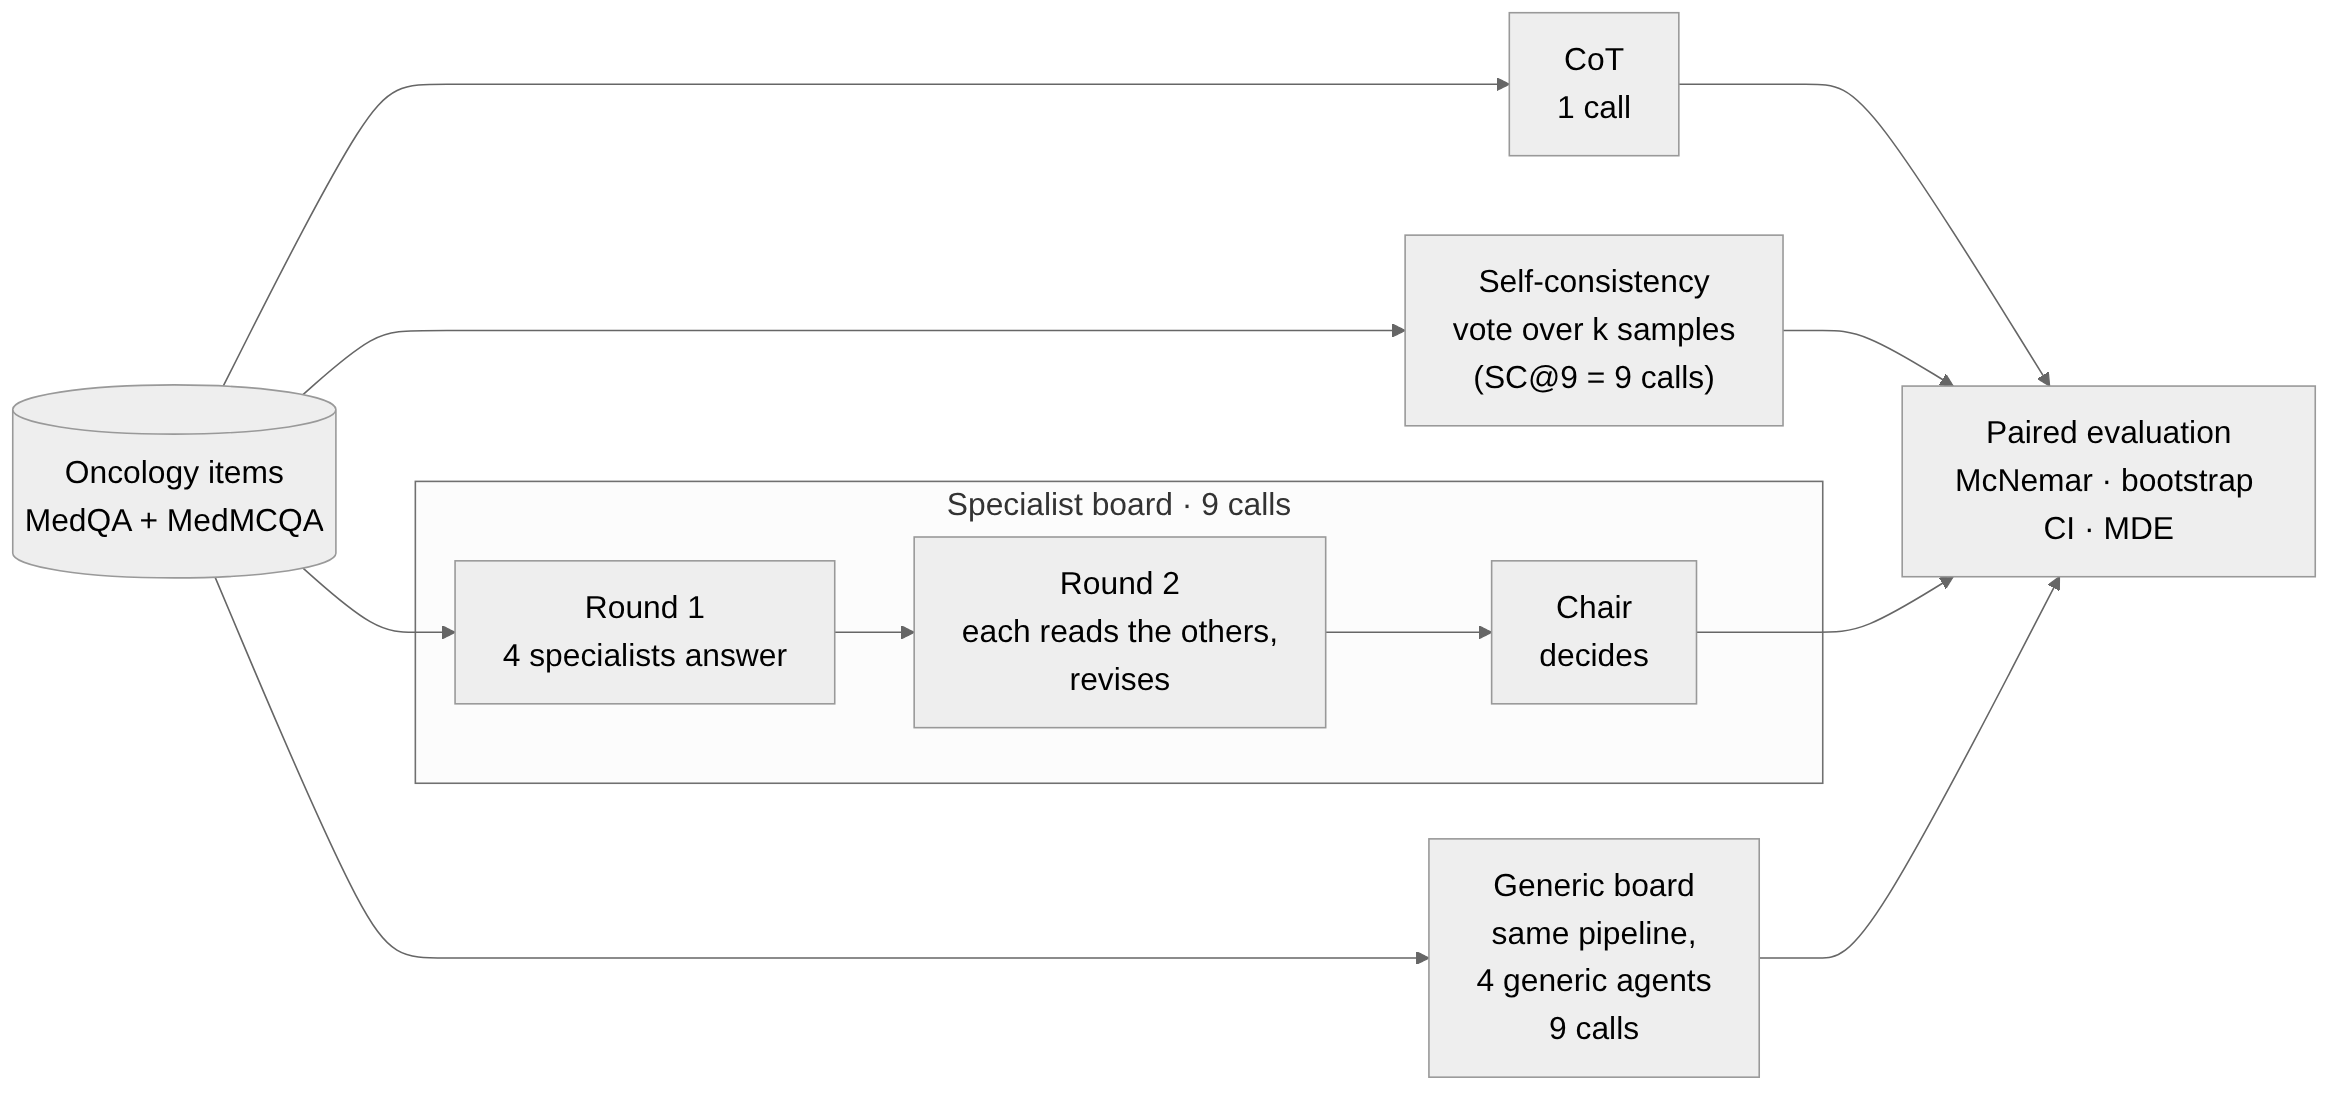
\includegraphics[width=0.85\textwidth]{figures/pipeline_paper.png}
\caption{Study pipeline (protocol v1.2). All arms share the model, prompt format, sampling settings and parser. CoT uses 1 call per item; SC@9, the specialist board and the generic board use 9.}
\label{fig:arch}
\end{figure*}

\subsection{Statistical analysis}
The primary comparison is specialist board versus SC@9 on the primary set (seed 0), with an exact two-sided McNemar test~\cite{mcnemar1947} at $\alpha=0.05$. A difference is called meaningful only if it is significant \emph{and} at least 2 percentage points. Three secondary comparisons are Holm-adjusted as one family~\cite{holm1979}: specialist vs generic board, round-2 vote vs round-1 vote, and specialist board vs CoT. Accuracy differences carry 95\% paired item-bootstrap intervals (10{,}000 resamples). For each non-significant comparison we report the smallest difference the test could detect with 80\% power, computed exactly from $n$ and the observed share of discordant items. Member answer changes from round~1 to round~2 are summarised as correct$\to$wrong and wrong$\to$correct rates, with intervals from resampling items. Unparseable answers count as wrong, and parse-failure and truncation rates are reported per arm. Matching calls does not match tokens: board members in round~2 and the chair read the other agents' texts. We therefore report API-equivalent tokens per item for every comparison, and add a pre-registered exploratory comparison against SC@15, a higher-budget sampling arm.

\section{Experimental Setup}
The model is Qwen2.5-7B-Instruct~\cite{qwen2025qwen25} (Apache-2.0) served with vLLM~\cite{kwon2023vllm} in fp16 on two NVIDIA T4 GPUs (Kaggle) \toverify{hardware and library versions from the run logs}. Seeds 0, 1 and 2 are run on the primary set and seed~0 on the secondary set; seed~0 was pre-registered as the primary analysis and the other seeds are reported as sensitivity. Every call's seed is derived from the run seed, item and role. The protocol, including datasets, comparisons, thresholds and seed plan, was frozen before any model output (version 1.2; the change from 1.1 added the SC@15 comparison and was made before any run). Runs were gated on four checks: an overlap check between debugging and test items, a smoke test, parse failures of at most 3\%, and CoT accuracy above the accuracy of always choosing the most frequent correct letter (27.8\% on the MedQA oncology subset; \toverify{MedMCQA floor}). Prompts were developed only on 20 MedQA training items. Code, configuration and logs are available in the project repository \toverify{public repository URL}.

\section{Results}
\pending{All results. Tables~\ref{tab:main} and~\ref{tab:comparisons} are generated from \texttt{results/} by \texttt{scripts/make\_paper\_tables.py}; nothing is typed by hand.}
% AUTO-GENERATED by scripts/make_paper_tables.py --pending. No real results exist yet.
\begin{table}[t]
\centering\small
\caption{Main results on the primary oncology set (seed 0). \textbf{PENDING: no real model output yet.}}
\label{tab:main}
\begin{tabular}{lrcc}
\toprule
Method & Calls & Acc. (95\% CI) & $\Delta$ vs SC@9 \\
\midrule
CoT (greedy) & 1 & -- & -- \\
SC@9 & 9 & -- & -- \\
Specialist board & 9 & -- & -- \\
Generic board & 9 & -- & -- \\
\bottomrule
\end{tabular}
\end{table}

\begin{table*}[t]
\centering\small
\caption{Pre-specified paired comparisons. \textbf{PENDING: no real model output yet.}}
\label{tab:comparisons}
\begin{tabular}{llrrrr}
\toprule
Role & Comparison & $\Delta$ (pp) & 95\% CI & $p_{\mathrm{Holm}}$ & MDE (pp) \\
\midrule
Primary & Specialist board vs SC@9 & -- & -- & -- & -- \\
Secondary & Specialist vs generic board & -- & -- & -- & -- \\
Secondary & Round-2 vote vs round-1 vote & -- & -- & -- & -- \\
Secondary & Specialist board vs CoT & -- & -- & -- & -- \\
\bottomrule
\end{tabular}
\end{table*}


\subsection{RQ1: specialist board vs self-consistency at equal calls}
\pending{difference, CI, $p$, MDE; reading per the pre-registered decision table}

\subsection{RQ2 and RQ3: roles and discussion}
\pending{role ablation; round-2 vs round-1 vote; correct$\to$wrong and wrong$\to$correct rates; chair overrides}

\subsection{Cost and robustness}
\pending{tokens and seconds per item; seeds 1--2; MedQA vs MedMCQA; stem-only and human-audited subsets}

\section{Discussion}
\pending{written only after results, following the interpretation plan fixed on 24 Oct 2026}

\section{Limitations}
Exam multiple-choice questions are a proxy for, not a sample of, tumor-board decisions: there are no patient records, images, pathology slides or guidelines in context. The oncology scope is defined by a keyword filter, so a human audit and a stem-only sensitivity set are reported alongside it. Only one 7B model is tested, so nothing generalises to other models. The MedQA oncology subset alone can detect only large differences (about 12--15 points with 80\% power), which is why sources are pooled and why every null is reported with its detectable effect. Public benchmarks may appear in the model's pre-training data. This affects all arms equally but inflates absolute accuracy. Finally, call matching equalises the number of calls, not tokens; token-matched readings are reported separately.

\section{Conclusion}
\pending{one paragraph, bounded to exam accuracy, this model and this budget}

\section*{AI assistance statement}
Claude (Anthropic) was used as a supervised research assistant: literature search and verification, gap analysis, code generation and debugging, test writing, statistical tooling and drafting. The bibliographic metadata of every reference was checked against its source; two literature statements taken from AI-generated summaries are marked for verification in the text. Every code path was run and tested, and every number in the results tables is generated from logged model outputs. The decisions, verification steps and AI errors that were caught are recorded in the project's decision log and AI-assistance report.

\IfFileExists{IEEEtran.bst}{\section*{Data availability and ethics}
All items come from public benchmarks (MedQA, MIT licence; MedMCQA, MIT licence). The model is released under Apache-2.0. No human participants or patient records were involved. Code, configuration, prompts and raw model outputs are released in the project repository \toverify{URL}.

\bibliographystyle{IEEEtran}}{\bibliographystyle{unsrt}}
\bibliography{references}
\end{document}
